\section{Fresnel single interface}

The first benchmark reduces the TMM to its simplest non-trivial case: a
single planar interface between two semi-infinite half-spaces, without any
finite layer at all. Light enters from air ($n_0 = 1.00$) onto a
bulk crown-glass substrate ($n_1 = 1.50$) at the fixed wavelength
$\lambda = \SI{550}{\nano\metre}$, and the angle of incidence $\theta_0$ is
swept from $0$ to \SI{89.9}{\degree} on a 901-point grid. Because there is
no finite layer, the TMM is called with an empty thickness list, and the
calculation collapses algebraically to the Fresnel amplitude coefficients
\begin{align}
  r_s &= \frac{n_0\cos\theta_0 - n_1\cos\theta_1}{n_0\cos\theta_0 + n_1\cos\theta_1}, \label{eq:fresnel-rs}\\[2pt]
  r_p &= \frac{n_1\cos\theta_0 - n_0\cos\theta_1}{n_1\cos\theta_0 + n_0\cos\theta_1}, \label{eq:fresnel-rp}
\end{align}
with Snell's law $n_0\sin\theta_0 = n_1\sin\theta_1$ fixing the refraction
angle. The code uses the sign convention in which $r_s(0) = r_p(0)$ at
normal incidence; the formulas~\eqref{eq:fresnel-rs}--\eqref{eq:fresnel-rp}
stated in the usual Wikipedia form give $r_s(0) = -r_p(0)$, so they differ
from the code by an overall sign in $r_p$ only, which leaves $|r_p|^{2}$
and hence the reflectance unchanged. The Brewster angle at which $r_p$
vanishes follows from~\eqref{eq:fresnel-rp} as
$\theta_B = \arctan(n_1/n_0) = \SI{56.31}{\degree}$.

\begin{center}
\begin{tikzpicture}
  \fill[black!4] (0,0) rectangle (5,1.8);
  \fill[blue!6]  (0,-1.2) rectangle (5,0);
  \draw[thick] (0,0) -- (5,0);
  \node[lbl, anchor=east] at (4.9, 1.4) {$n_0$ (air)};
  \node[lbl, anchor=east] at (4.9,-0.8) {$n_1$ (glass)};
  \raysketch{1.6}{35}{f}
\end{tikzpicture}
\end{center}

\begin{figure}[!htbp]
  \centering
  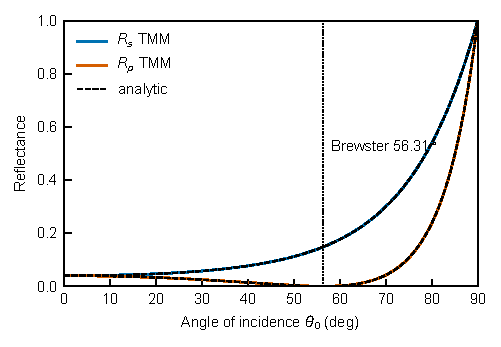
\includegraphics[width=0.5\textwidth]{01_fresnel_single_interface.pdf}
  \caption{Reflectance of an air/glass interface at \SI{550}{\nano\metre} for $s$- and $p$-polarisation. TMM (colour) coincides with the closed-form Fresnel result (dashed) at machine precision. The Brewster angle is marked by the dotted vertical line.}
  \label{fig:fresnel-single}
\end{figure}

The TMM reproduces the closed-form reflectance to
$\max|\Delta R| \approx \num{4e-13}$ across the full sweep, and
$|r_p(\theta_B)| \approx \num{3e-16}$ exactly at the Brewster angle. Both
residuals are at the level of double-precision floating-point noise, which
confirms that the single-interface coefficients are evaluated correctly
before any multilayer machinery is invoked.


